\section{Blockchain}
\subsection{Khái niệm Blockchain}

Blockchain là một công nghệ mới và đầy tiềm năng, được sử dụng để lưu 
trữ và quản lý thông tin một cách an toàn và minh bạch. Nó là một cơ 
sở dữ liệu phân tán, trong đó dữ liệu được lưu trữ trên nhiều nút 
mạng và được bảo vệ bởi mã hóa mạnh. Cơ sở dữ liệu này sẽ lưu thông tin trong các khối (block), các khối 
này sẽ được liên kết với nhau bằng mã hóa và có thể mở rộng theo 
thời gian để tạo thành chuỗi (chain).Vì vậy, 
nếu một block bị thay đổi hoặc xóa, toàn bộ blockchain sẽ bị ảnh 
hưởng và trở nên không hợp lệ.

Ta có thể hiểu đơn giản Blockchain chính là một cuốn sổ cái kỹ thuật 
số phân tán. Cuốn sổ cái này sẽ lưu trữ tất cả các loại thông tin 
giao dịch và được sao chép thành nhiều bản đặt tại nhiều máy tính khác nhau. 

Không giống như các cơ sở dữ liệu thông thường, blockchain là cơ sở dữ liệu phi tập trung. 
Tức là blockchain không được đặt tại một vị trí và chịu sự quản lý của một quản trị viên. 
Thay vào đó, nó được sao chép thành nhiều bản và được lưu trên các máy tính riêng lẻ gọi là nút. 


Blockchain được sử dụng cho nhiều mục đích khác nhau, bao gồm việc 
lưu trữ tiền điện tử và các giao dịch tài chính, quản lý thông tin 
y tế, quản lý lưu trữ dữ liệu và cung cấp giải pháp cho việc xác 
thực danh tính và bảo mật thông tin.

Một trong những ưu điểm của blockchain là tính minh bạch và an toàn. 
Do dữ liệu được lưu trữ phân tán, không ai có thể can thiệp vào và 
thay đổi dữ liệu một cách dễ dàng. Ngoài ra, blockchain cũng giúp 
giảm thiểu sự phụ thuộc vào các bên trung gian và giảm chi phí cho 
việc tạo ra và quản lý các hệ thống tương tự.

Tuy nhiên, cũng có những hạn chế của blockchain, bao gồm tốc độ xử 
lý chậm và khó khăn trong việc thay đổi các thông tin đã được lưu 
trữ trên blockchain. Tuy nhiên, với sự phát triển và ứng dụng đa 
dạng, blockchain đang trở thành một công nghệ quan trọng và tiềm 
năng cho tương lai.
\subsection{Hệ thống phi tập chung}

Ở phần \textbf{4.1}, chúng ta nói rằng Blockchain là một hệ thống 
phi tập trung. Vậy hệ thống phi tập trung khác hệ thống tập trung
như thế nào?

\begin{figure}[h]
    \centering
    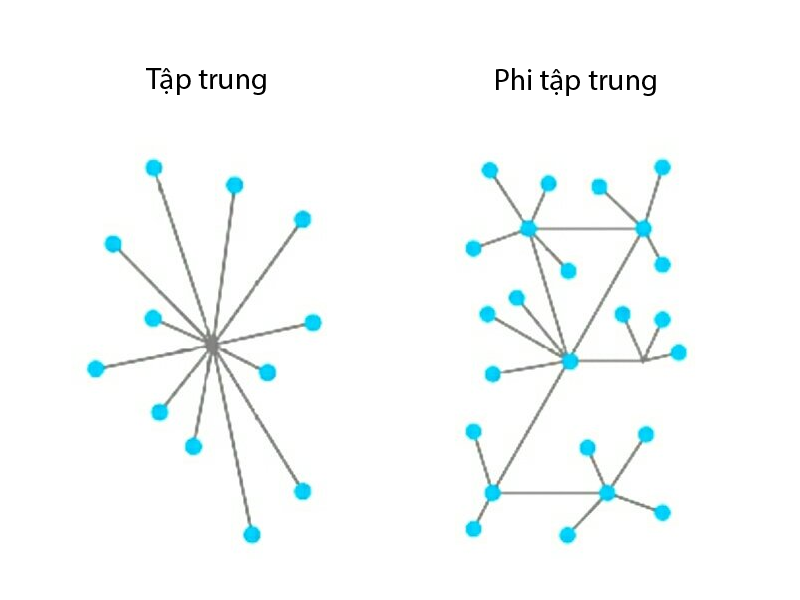
\includegraphics[width=0.7\textwidth]{images/He_thong_tap_chung:phi_tap_chung.png}
    \label{fig:He_thong_tap_chung/phi_tap_chung}
    \caption{Hệ thống tập trung và phi tập trung}
\end{figure}

Hệ thống tập trung là một hệ thống mà tất cả các thành phần của nó
được đặt tại một vị trí và chịu sự quản lý của một quản trị viên.
Ví dụ như hệ thống quản lý thông tin của một công ty, hệ thống
quản lý thông tin của một trường học, hệ thống quản lý thông tin
của một bệnh viện, hệ thống quản lý thông tin của một ngân hàng
v.v...

Hệ thống phi tập trung là một hệ thống mà không có bên nào kiểm soát 
toàn bộ. Trong hệ thống này, tất cả các thực thể trong hệ thống là 
ngang hàng. Các quyết định và hoạt động được phân phối trên nhiều 
thực thể độc lập và được quyết định bởi một cộng đồng người dùng.

Ưu điểm của hệ thống phi tập chung là dữ liệu sẽ được đảm bảo, 
không bị thay đổi, không bị xóa bỏ. Hệ thống phi tập chung đảm bảo
tính minh bạch, an toàn, độ tin cậy và khả năng phát triển dễ dàng.. 
Tuy nhiên, tốc độ xử lý chậm và khó khăn trong việc đạt được sự đồng
thuận giữa các thực thể phân tán là những vấn đề cần giải quyết để 
hế thống phát triển mạnh mẽ hơn.

\subsection{Cấu tạo của blockchain}

Blockchain là một cấu trúc dữ liệu phân tán, bao gồm nhiều block được kết nối với nhau thông qua các liên kết mã hóa. Mỗi block chứa thông tin về một số giao dịch được thực hiện trên mạng blockchain.

Một blockchain cơ bản bao gồm các thành phần sau:

Hash: là một mã hóa duy nhất đại diện cho một block hoặc một tập hợp các thông tin trên blockchain. Hash được tạo ra bằng cách sử dụng một thuật toán mã hóa, chẳng hạn như SHA-256.

Block: là một đơn vị cơ bản của blockchain, chứa thông tin về các giao dịch và các liên kết đến các block khác trong chuỗi.

Chuỗi block (blockchain): là một loạt các block được kết nối với nhau theo thứ tự thời gian. Mỗi block trong chuỗi chứa liên kết đến block trước đó và block sau đó, tạo thành một chuỗi liên kết.

Proof of work (POW): là một phương thức để xác minh và chứng thực các giao dịch trên blockchain. POW yêu cầu các nút mạng phải giải quyết một bài toán toán học khó để thêm một block mới vào blockchain, đồng thời cũng giúp bảo vệ blockchain khỏi các cuộc tấn công.

Node: là một thiết bị hoặc một phần mềm chạy trên thiết bị, được sử dụng để tham gia vào mạng blockchain, giúp xác minh và chứng thực các giao dịch.

Wallet: là một phần mềm hoặc thiết bị lưu trữ khóa cá nhân và khóa công khai, cho phép người dùng thực hiện các giao dịch trên mạng blockchain.

Các thành phần này cùng hoạt động để tạo ra một hệ thống blockchain an toàn, minh bạch và phân tán, giúp các giao dịch trên mạng blockchain được xác minh và chứng thực một cách chính xác.

\subsection{Cấu tạo của Blockchain}

Một blockchain cơ bản bao gồm các thành phần sau:
\begin{itemize}
    \item[-] Hash: là một mã băm duy nhất đại diện cho một block hoặc một tập hợp các thông tin trên blockchain. Hash được tạo ra bằng cách sử dụng một thuật toán băm, chẳng hạn như SHA-256.
    \item[-] Block (Khối): là một đơn vị cơ bản của blockchain, chứa thông tin về các giao dịch và các liên kết đến các block khác trong chuỗi.
    \item[-] Chuỗi block (blockchain): là một loạt các block được kết nối với nhau theo thứ tự thời gian. Mỗi block trong chuỗi chứa liên kết đến block trước đó và block sau đó, tạo thành một chuỗi liên kết.
    \item[-] Proof of work (POW): là một phương thức để xác minh và chứng thực các giao dịch trên blockchain. POW yêu cầu các nút mạng phải giải quyết một bài toán toán học khó để thêm một block mới vào blockchain, đồng thời cũng giúp bảo vệ blockchain khỏi các cuộc tấn công.
    \item[-] Node: là một thiết bị hoặc một phần mềm chạy trên thiết bị, được sử dụng để tham gia vào mạng blockchain, giúp xác minh và chứng thực các giao dịch.
    \item[-] Wallet: là một phần mềm hoặc thiết bị lưu trữ khóa cá nhân và khóa công khai, cho phép người dùng thực hiện các giao dịch trên mạng blockchain.

\end{itemize}


Các thành phần này cùng hoạt động để tạo ra một hệ thống blockchain an toàn, minh bạch và phân tán, giúp các giao dịch trên mạng blockchain được xác minh và chứng thực một cách chính xác.

\subsubsection{Cấu trúc của một khối}


Cấu trúc của 1 khối (block) được minh hoạ qua sơ đồ sau:
\begin{figure}[h]
    \centering
    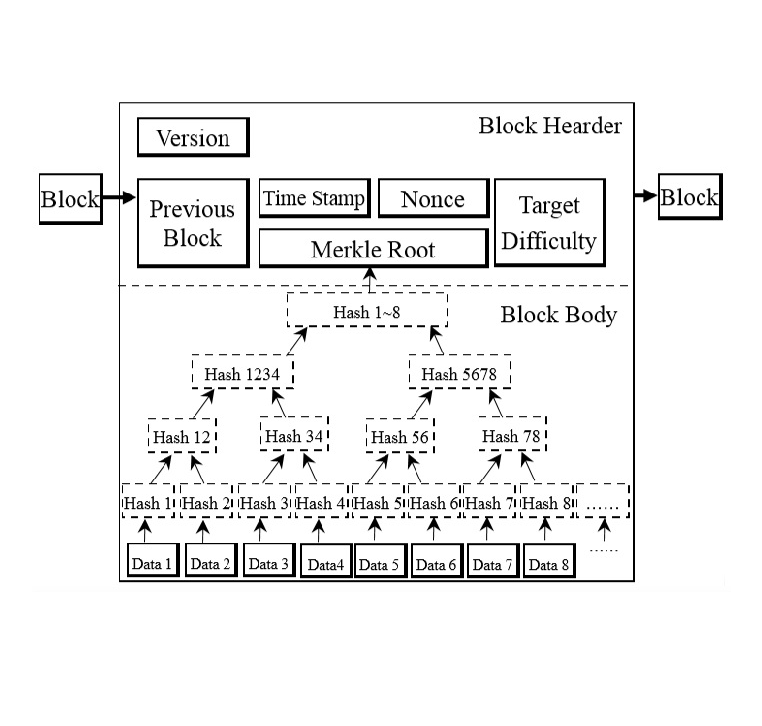
\includegraphics[width=0.7\textwidth]{images/Cau_truc_khoi.png}
    \label{fig:cau_truc_khoi}
    \caption{}
\end{figure}

\begin{itemize}
    \item[-] Block header: chứa các thông tin về block, bao gồm: thời gian tạo block, hash của block trước đó, hash của block hiện tại, nonce, và các thông tin khác.
    \begin{itemize}
        \item[+] Version: phiên bản của blockchain.
        \item[+] Previous Block: Giá trị băm của block trước.
        \item[+] Time Stamp: Thời gian block này được tạo.
        \item[+] Merkle Root: Mã hash của tất cả các giao dịch trong khối hiện tại, 
        được tính toán bằng cách sử dụng cây Merkle.
        \item[+] Nonce: là một số ngẫu nhiên được sử dụng để giải quyết bài toán PoW.
        \item[+] Target Difficulty: là một giá trị được sử dụng để xác định độ khó của bài toán PoW trong block này.
    \end{itemize}
    \item[-] Transaction: là các giao dịch được thực hiện trên blockchain.
\end{itemize}

\subsection{Các kỹ thuật trong Blockchain}
\subsubsection{Cấu trúc phi tập trung}
Cấu trúc phi tập chung (decentralized structure) trong blockchain được xây dựng 
để đảm bảo tính an toàn và bảo mật của hệ thống. Cấu trúc này cho phép thông tin được phân tán trên nhiều nút mạng khác nhau, giúp giảm thiểu rủi ro bị tấn công và tăng tính đáng tin cậy.

Cấu trúc phi tập chung trong blockchain có có thành phần cơ bản như:
\begin{itemize}
    \item[-] Mạng ngang hàng (peer-to-peer network): Các nút trong mạng sẽ kết 
    nối với nhau để chia sẻ thông tin và cập nhật các giao dịch mới nhất.
    \item[-] Giao thức đồng thuận (consensus protocol): Để đảm bảo tính nhất 
    quán và đáng tin cậy của dữ liệu, các nút trong mạng sẽ phải đồng thuận về 
    sự thay đổi của blockchain. Các giao thức đồng thuận phổ biến bao gồm Proof 
    of Work (PoW) và Proof of Stake (PoS).
    \item[-] Các thợ mỏ (miners): Các thợ mỏ sẽ đóng vai trò giải quyết các
    phép tính phức tạp để đào ra các khối mới và xác nhận các giao dịch.
    \item[-] Blockchain: Dữ liệu được lưu trữ trên blockchain, một chuỗi
    các khối được kết nối với nhau theo thứ tự thời gian.
    \item[-] Wallet: là một phần mềm hoặc thiết bị lưu trữ khóa cá nhân và
    khóa công khai, cho phép người dùng thực hiện các giao dịch trên mạng
    blockchain.
\end{itemize}

Các thành phần này cùng hoạt động với nhau để tạo ra một hệ thống phi tập trung, 
nơi mà dữ liệu được phân tán trên nhiều nút khác nhau và không có bất kỳ cơ quan 
trung gian nào kiểm soát hoặc giám sát.

\subsubsection{Tính tin cậy}
Tính tin cậy (reliability) là một trong những điểm mạnh của blockchain. Điều 
này được đảm bảo bởi cấu trúc phi tập trung của hệ thống, nghĩa là không có 
một tổ chức hay cá nhân nào có quyền kiểm soát toàn bộ blockchain. Thay vào đó, 
blockchain được phân tán trên nhiều nút trong mạng, mỗi nút lưu trữ một bản sao 
của toàn bộ blockchain.

Việc phân tán dữ liệu trên nhiều nút khác nhau giúp tăng tính đáng tin cậy của 
hệ thống, vì không có một nút duy nhất nào có thể gian lận hoặc tấn công hệ 
thống. Nếu một nút bị tấn công hoặc lỗi, các nút khác vẫn có thể tiếp tục 
hoạt động và duy trì tính toàn vẹn của blockchain.

Trao đổi dữ liệu giữa các nút không yêu cầu sự tin tưởng lẫn nhau. Quy chế 
hoạt động của hệ thống và dữ liệu được công khai 
và minh bạch, vì thế các nút không thể giả mạo các quy tắc và thời gian được 
chỉ định bởi hệ thống.
\subsubsection{Giao thức đồng thuận}
\begin{itemize}
    \item[-] \textbf{Proof of Work(PoW)}: có nhiệm vụ đảm bảo 
    tính nhất quán và đáng tin cậy của blockchain bằng cách yêu cầu các nút 
    trong mạng phải thực hiện một số lượng lớn tính toán để xác nhận giao dịch
    và thêm mới các khối vào blockchain. Cụ thể, các nút trong mạng sẽ cạnh 
    tranh với nhau để giải quyết một bài toán tính toán phức tạp, được gọi là 
    "bài toán đào". Bài toán này yêu cầu các nút phải tìm ra một giá trị hash 
    thoả mãn điều kiện, dựa trên các thông tin trong khối mới nhất và khối trước đó. 
    Việc giải quyết bài toán này đòi hỏi sự tiêu tốn của năng lượng tính toán, 
    thời gian và tài nguyên máy tính. Điều kiện này là giá trị “difficulty” – 
    số lượng số 0 đứng phía trước giá trị băm.
    \item[-] \textbf{Proof of Stake(PoS)}: là một giao thức đồng thuận được sử 
    dụng trong blockchain để đảm bảo tính nhất quán và đáng tin cậy của dữ 
    liệu. PoS hoạt động khác với PoW, bằng cách không yêu cầu các nút trong 
    mạng thực hiện các hoạt động tính toán phức tạp để giải quyết bài toán đào, 
    mà thay vào đó, các nút sẽ được chọn để xác nhận giao dịch và thêm mới các 
    khối vào blockchain dựa trên số lượng tiền điện tử mà họ đã có trong tài 
    khoản của mình.
    
\end{itemize}


Blockchain sử dụng các giao thức đồng thuận để đảm tính tin cậy và bảo mật. Khi không nắm được 51\% 
số nút trong mạng, dữ liệu mạng không thể bị kiểm soát và sửa đổi. Do đó, 
bản thân Blockchain đã trở nên tương đối an toàn và có thể tránh việc sửa đổi 
dữ liệu. Vì thế, nếu một số lượng lớn các nút có khả năng tính toán mạnh được 
tham gia vào hệ thống thì dữ liệu trong hệ thống này sẽ có độ bảo mật cao hơn.  



\subsection{Cách thức hoạt động của Blockchain}
\subsubsection{Thêm giao dịch mới vào Blockchain}
Để thêm một giao dịch trong blockchain, quá trình cần phải đi qua các bước sau:
\begin{itemize}
    \item[-] Người dùng gửi một thông tin của giao dịch mới vào mạng blockchain.
    \item[-] Giao dịch mới sẽ được gửi đến tất cả các nút trong mạng blockchain.
    \item[-] Các nút trong mạng sẽ kiểm tra tính hợp lệ của giao dịch bằng cách kiểm tra tính 
    đúng đắn của chữ ký số.
    \item[-] Các giao dịch hợp lệ sẽ được đóng gói lại thành một khối và bao gồm các thông tin 
    như mã băm của khối trước, thông tin của giao dịch, phiên bản, thời gian tạo khối,... 
    \item[-] Tính toán giá trị hash của block mới, các nút trong mạng sẽ xác nhận tính hợp 
    lệ của khối mới. Để xác nhận, các nút sẽ kiểm tra giá trị hash của khối trước đó có khớp 
    với giá trị Previous Hash được lưu trong khối mới hay không. Tiếp theo, sẽ kiểm tra Merkle Root
    của khối mới có khớp với giá trị Merkle Root được lưu trong khối mới hay không. Cuối cùng sẽ 
    kiểm tra thời gian tạo khối, giá trị nonce. 
    \item[-] Nếu khối mới được xác nhận là hợp lệ, nó sẽ được thêm vào blockchain. Khối mới này sẽ trở thành khối mới nhất trong chuỗi blockchain và các giao dịch được bao gồm trong khối sẽ được coi là đã được xác nhận và lưu trữ vĩnh viễn trong blockchain.
\end{itemize}

\subsubsection{Xác thực một giao dịch}
\begin{itemize}
    \item[-] Tính mã băm của giao dịch cần xác thực
    \item[-] Tìm tất cả các khối trong chuỗi khối (blockchain) và kiểm tra xem mã băm của giao 
    dịch đó có nằm trong danh sách các giao dịch của mỗi khối hay không.
    Nếu không tồn tại thì thông tin giao dịch là sai.
    \item[-] Nếu có thì kiểm tra tính toàn vẹn của giao dịch bằng cách sử dụng chữ ký số 
    của người gửi giao dịch.
        \item[+] Sử dụng khoá công khai để giải mã chữ ký số.
        \item[+] Tính toán lại mã băm (hash) của dữ liệu giao dịch bằng cách sử dụng cùng
        thuật toán mã hóa được sử dụng trong blockchain 
        \item[+] So sánh hai giá trị vừa tính được. Nếu trùng khớp thì giao dịch được
        xác nhận là hợp lệ và tính toàn vẹn của giao dịch được xác định.
        Việc xác minh tính toàn vẹn trên dựa vào thuật toán Chữ ký số trên đường cong 
        elliptic (ECDSA) đã được chứng minh ở phần \textbf{2.4.2}
\end{itemize}

\subsection{Các ứng dụng điển hình của Blockchain}
\subsubsection{Tiền số}

Tiền số trong blockchain là một loại tiền tệ số được tạo ra và quản lý bởi các 
mạng blockchain, được mã hóa để đảm bảo tính bảo mật và độ tin cậy của các giao 
dịch trên mạng. Các ví dụ tiêu biểu của tiền số trên thế giới hiện nay bao gồm 
Bitcoin, Ethereum, Litecoin, Ripple và Bitcoin Cash. Mỗi loại tiền số có đặc điểm 
và tính năng riêng, tuy nhiên tất cả đều được tạo ra và quản lý bởi các mạng 
blockchain. Tiền số trong blockchain có tính năng phân quyền, không có bên trung 
gian nào can thiệp hoặc kiểm soát quá trình giao dịch và các giao dịch được xác 
thực bởi các nút trong mạng. Tiền số trong blockchain được sử dụng trong nhiều 
ứng dụng như chuyển tiền, thanh toán trực tuyến, đầu tư và trao đổi trên các sàn 
giao dịch tiền số, tuy nhiên, nó cũng đang gặp phải một số thách thức như tính 
ổn định giá, độ tin cậy và sự phức tạp về quy định pháp lý.

\subsubsection{Hợp đồng thông minh} 

Hợp đồng thông minh (smart contract) là một chương trình tự động được viết bằng ngôn ngữ lập trình và thực thi trên mạng blockchain. Chúng được thiết kế để tự động thực hiện các điều khoản hợp đồng một cách đáng tin cậy, không cần phải dựa vào bên thứ ba.

Hợp đồng thông minh được định nghĩa bởi một tập hợp các quy tắc và điều kiện mà khi được kích hoạt, nó sẽ tự động thực hiện các hành động được yêu cầu. Các hợp đồng thông minh được sử dụng để thực hiện các giao dịch tài chính, quản lý quy trình kinh doanh, bảo vệ sở hữu trí tuệ và quản lý dữ liệu.

Một trong những đặc điểm của hợp đồng thông minh là tính bảo mật cao, vì chúng được mã hóa và lưu trữ trên mạng blockchain, không thể bị can thiệp hay thay đổi bởi bất kỳ ai. Các giao dịch được thực hiện thông qua các hợp đồng thông minh cũng được xác thực và đảm bảo tính đúng đắn bởi các nút trong mạng.

Hợp đồng thông minh đã được triển khai trong nhiều lĩnh vực, bao gồm tài chính, bảo hiểm, bất động sản, quản lý chuỗi cung ứng và nhiều lĩnh vực khác. Tuy nhiên, việc triển khai hợp đồng thông minh vẫn đang đối mặt với một số thách thức, bao gồm khả năng lập trình và kiểm tra hợp đồng, độ tin cậy và quy định pháp lý.